\section{Experimentkonfiguration}\label{section:prototypische-implementierung:experimentkonfiguration}

Um die in \autoref{section:konzeption:experimentkonfiguration} beschriebene Experimentkonfiguration für die prototypische Implementierung nutzen zu können, wurden neben der IDE auch eine entsprechende Steuereinheit sowie ein steuerbares Laborgerät entwickelt. Die genaue Implementierung und Anbindung dieser innerhalb des Experiments werden im Folgenden dargelegt.

\paragraph{Steuereinheit}
Für die Implementierung der Steuereinheit wurde eine Simulation des AVR Microcontroller ATmega2560 \cite{noauthor_atmega2560_nodate} eingesetzt. Dabei wurde simavr \cite{pollet_simavr_2025} für die Simulation verwendet. Weiterhin wurde ein entsprechendes Node.js Addon geschrieben, welches den Zugriff auf die Simulation von einem Node.js Programm aus ermöglicht. Dadurch können die Werte der Pins über einen entsprechenden CrossLab-Service verändert und mit anderen Laborgeräten ausgetauscht werden. Bei diesem CrossLab-Service handelt es sich in der prototypischen Implementierung um den bereits vorhandenen \textit{Electrical Connection Service}, welcher als Prosumer verwendet wird. Die weiteren CrossLab-Services der Steuereinheit werden in den nachfolgenden Abschnitten betrachtet. Die Steuereinheit ist als ein cloud-instanziierbares Laborgerät implementiert.

\begin{figure}[tbp]
    \centering
    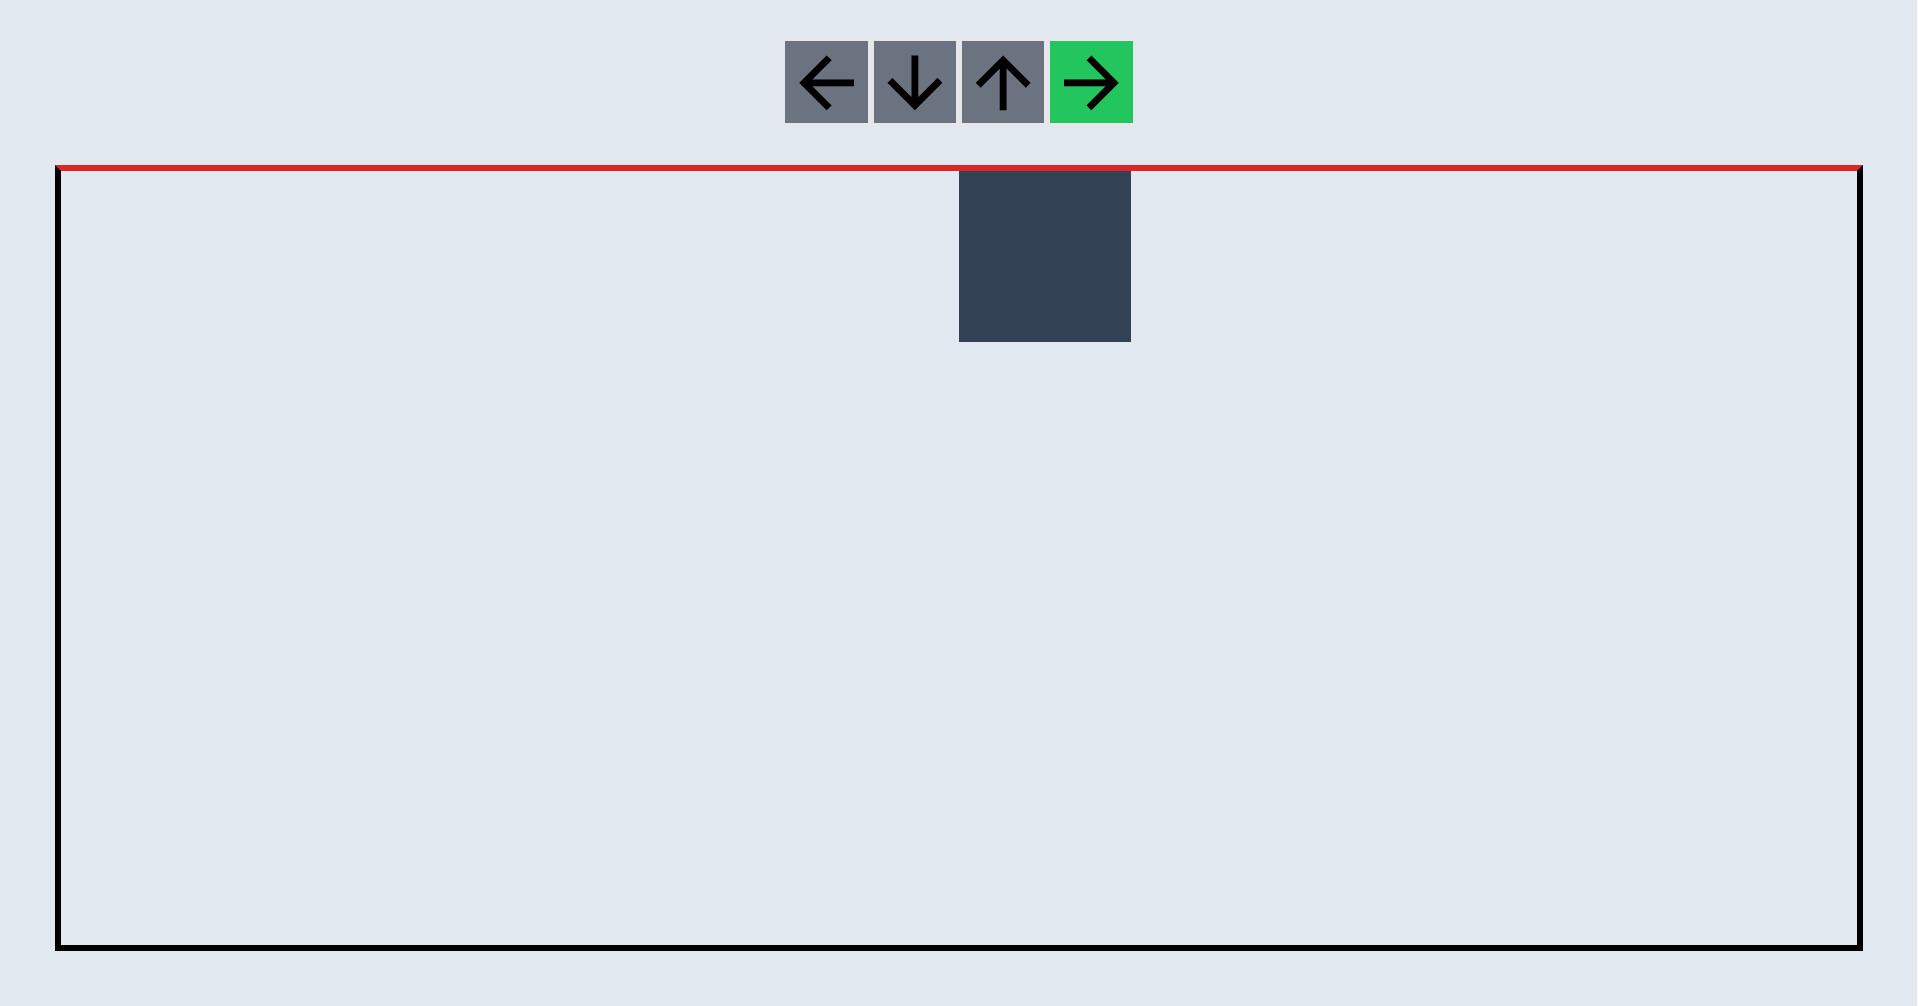
\includegraphics[trim={0 3px 0 0},clip,width=\textwidth]{images/vpspu.png}
    \caption{Virtuelles steuerbares Laborgerät}
    \label{figure:vpspu}
\end{figure}

\paragraph{Steuerbares Laborgerät}
Für die Implementierung des steuerbaren Laborgeräts wurde ein einfaches Programm entwickelt, welches die Steuerung eines Blocks innerhalb einer Box ermöglicht. Dieses ist in \autoref{figure:vpspu} dargestellt. Die Steuerung erfolgt über die Bereitstellung von digitalen Sensoren und Aktoren mithilfe eines Electrical Connection Service Prosumer. Dabei stehen Sensoren für die Ränder der Box bereit. Sollte sich der Block an einem der Ränder befinden, wird der Wert des Sensors auf \texttt{1} gesetzt, ansonsten auf \texttt{0}. Die Aktoren ermöglichen die Bewegung des Blocks nach links, rechts, oben und unten. Das steuerbare Laborgerät ist als ein edge-instanziierbares Laborgerät implementiert.

Somit besteht die betrachtete Experimentkonfiguration zunächst aus der IDE, der Steuereinheit und dem steuerbaren Laborgerät. Dabei wird die Steuereinheit über den Electrical Connection Service mit dem steuerbaren Laborgerät verbunden. Die IDE besitzt zunächst keine Verbindungen. Weitere Laborgeräte, CrossLab-Services und Verbindungen werden in den nachfolgenden Abschnitten hinzugefügt.